\documentclass{article}
\usepackage{graphicx}
\usepackage{cite}

\begin{document}
\title{Visual Tweets Sentimental Analysis}
\author{Lilong Jiang (jiang.573)}
\maketitle

\section{Introduction}
In this project, I build a visual online tweets sentimental analysis tool, which allows users to do the sentimental analysis for a certain topic. I also implement two classifiers and compare both classifiers over the performance and accuracy. 
\section{Dataset}
We get our datset from the Sentiment140\footnote{\texttt{\scriptsize{http://www.sentiment140.com/‎}}}. The training dataset in this dataset is collected by the Twitter API, whose content contains the emoticons :) and :(. The test dataset in this dataset is manually annotated.
\section{Preprocessing}
There are several challenges for the tweets processing: firstly, the tweets are very short, limited as 140 characters. Secondly, the tweets are very sloppy and it contains a lot of misspellings, slangs, abbreviations, emoticons, urls, etc. So the preprocessing step is very important for the later classification.
We preprocess all the tweets as follows: \\
(1) Remove usernames and urls. \\
(2) I use an emoticon dictionary ~\cite{agarwal2011sentiment}, in which each emoticon is labeled as emotion(positive or negative). The emoticons in the tweets are replaced by happy or sad. \\
(3) Replace all sequences of repeated characters by three characters, for example, convert goooood to goood.\\
(4) Expand abbreviations with a dictionary\footnote{\texttt{\scriptsize{http://www.noslang.com/‎‎}}}. For example, lol is converted into laughing out loud. \\
(5) NLTK\footnote{\texttt{\scriptsize{http://www.nltk.org/‎‎}}} is used to tokenize the tweet, remove the stop words, punctuations, and do the lemmatization. \\
(6) PyEnchant\footnote{\texttt{\scriptsize{http://pythonhosted.org/pyenchant/‎‎}}} is used to check whether the token is a correct English word. Only correct English words are retained.\\ 
\section{Classifiers}
Two classifiers are implemented in this project. One is the naive Bayes classifier and the other is the SVM. 
\subsection{Naive Bayes Classifier}
The Naive Bayes classifier is a simple probalistic classifier which is based on Bayes theorem. Each tweet will be classified into the class with the highest posterior probability.

\begin{center}
$C_{map} = argmax_{c \in C} (log P(c) + \sum_{1 \le k \le n_d} log P(t_k |c))$ 
\end{center}

\noindent The conditional probability of a particular word given a class as the relative frequency of term t in documents belongs to class c in the multinomial naive bayes model while in the binarized multinomial naive bayes model, each term has the same frequency which is 1:

\begin{center}
$P(t|c) = \frac{T_{ct} + 1}{\sum_{t \in V}(T_{ct} + 1)} = \frac{T_{ct} + 1}{\sum_{t \in V}(T_{ct}) + B}$
\end{center}

\noindent where B is the number of documents. \\
I use add-one smoothing to address the problem that a particular word doesn't appear in a particular class. \\
\subsection{Feature Selection}
For the naive bayes classifier, I implement two feature selection methods. One is the frequency-based feature selection. The other is based on the mutual information.
\subsubsection{Frequency-based Feature Selection}
All the adverb and adjective tokens are retained since it is more related to the polarity and for the verb and noun tokens, only tokens whose frequency is greater than 4 are retained. 
\subsubsection{Mutual Information}
Mutual Information is used to measure how much a term t contributes to the class c.

\begin{center}
$I(U; C) = \frac{N_{11}}{N} \log_2 \frac{N N_{11}}{N_{1.}N_{.1}} + \frac{N_{01}}{N} \log_2 \frac{N N_{01}}{N_{0.}N_{.1}} + \frac{N_{10}}{N} \log_2 \frac{N N_{10}}{N_{1.}N_{.0}} + \frac{N_{00}}{N}\log_2 \frac{N N_{00}}{N_{0.}N_{.0}}$
\end{center}

\noindent where $N_{10}$ is the number of documents that contain t and are not in class c. $N_{11}$ is the number of documents that contain t and are in class c. $N_{01}$ is the number of documents that don't contain t and are in class c. $N_{00}$ is the number of documents that don't contain t and are not in class c. $N_{1.}$ is the number of documents that contain t. $N_{0.}$ is the number of documents that don't contain t. $N_{.0}$ is the number of documents which are not in class c. $N_{.1}$ is the number of documents in class c.\\
We use add-1 smoothing for each count to void the divided by 0.
\subsection{SVM Classifier}
Libsvm\footnote{\texttt{\scriptsize{http://www.csie.ntu.edu.tw/~cjlin/libsvm/‎‎}}} is a library which implemented SVM algorithm. Libsvm is used to classify the tweets. ‎I use C-SVM and set the parameter of the cost to 4.
\subsection{Experiment}
I compare these two classifier on the performance and accuracy. 359 tweets are used to test the classifier.
\subsubsection{Parameter Sensitivity}
Shrinking Size \\
I plot the accuracy of Bayes classifier with the changing of the shrinking ratio in the mutual information. The result is shown in Figure. As we can see 
\subsubsection{Performance}
\subsubsection{Accuracy}
\section{Online Sentimental Analysis}
\subsection{Architecture}

\begin{figure}
\centering
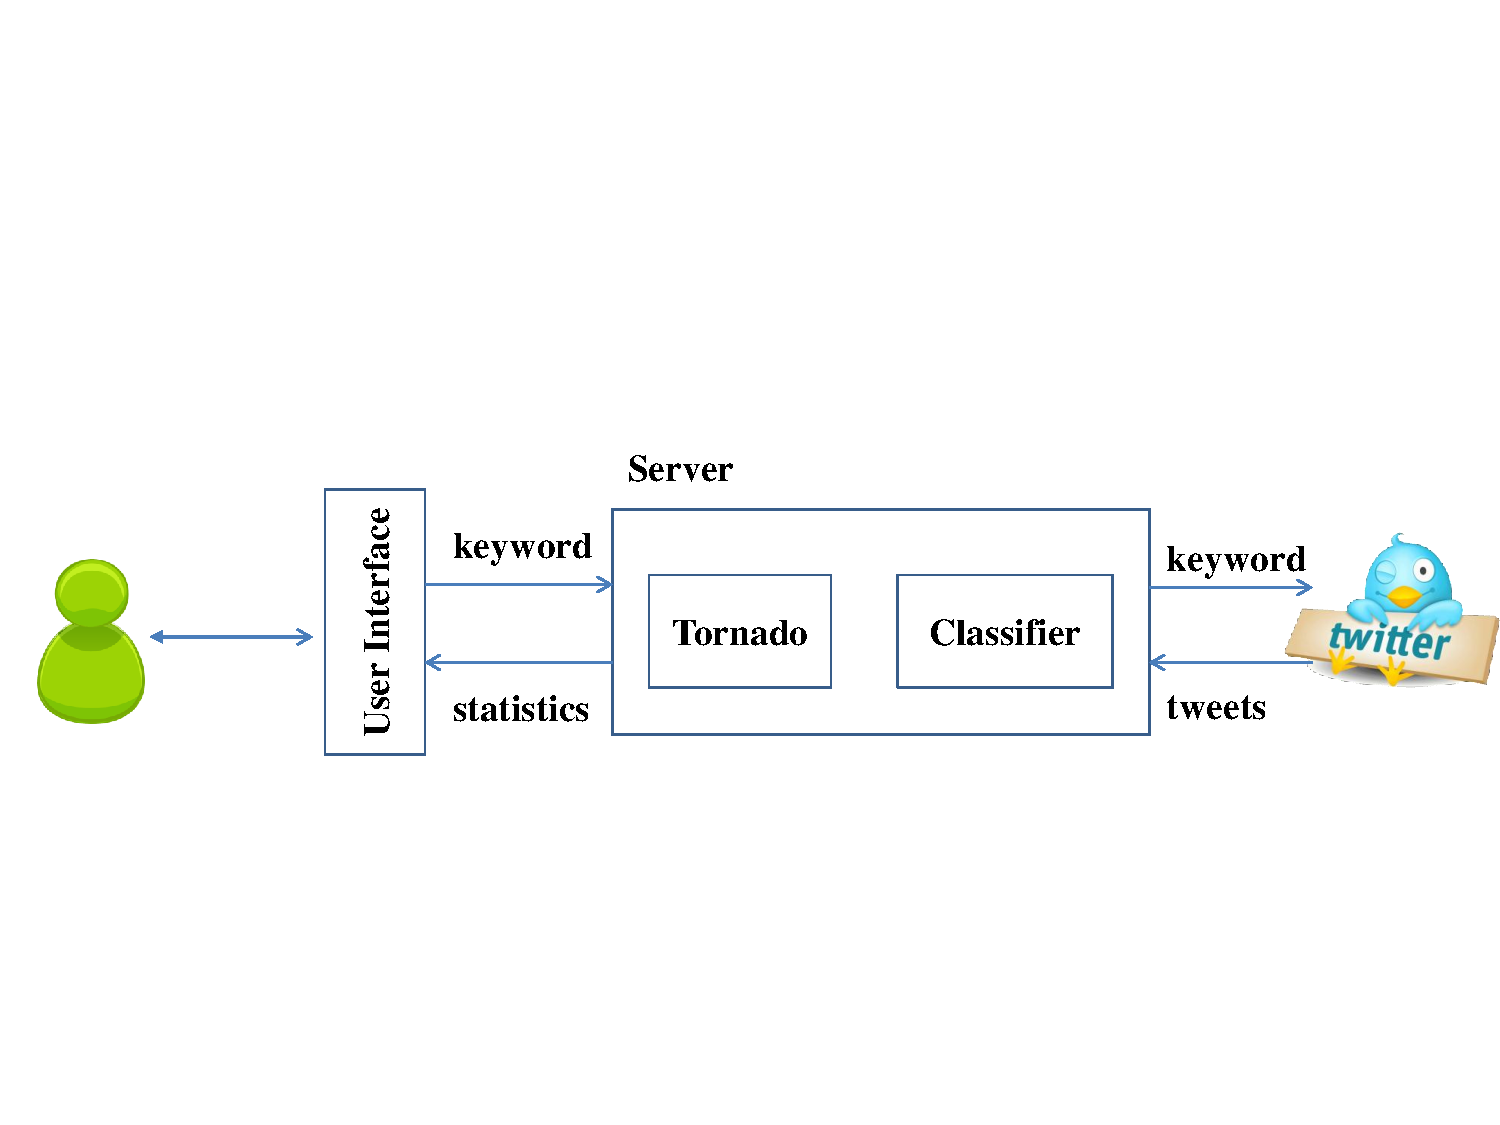
\includegraphics[width=0.8\textwidth]{pics/architecture.pdf}
\caption{Architecture}
\label{Fig:architecture}
\end{figure}

In the front end, D3\footnote{\texttt{\scriptsize{http://d3js.org/‎‎}}} is used to visualize the final result and Tornado\footnote{\texttt{\scriptsize{http://www.tornadoweb.org/}}} works as a web server. When users submit a topic, the server gets 500 tweets from twitter through twitter api and analyzes each tweet and returns the statistics information and tweets to the client. The user interface of this system is shown in Figure ~\ref{Fig:ui}.

\begin{figure}
\centering
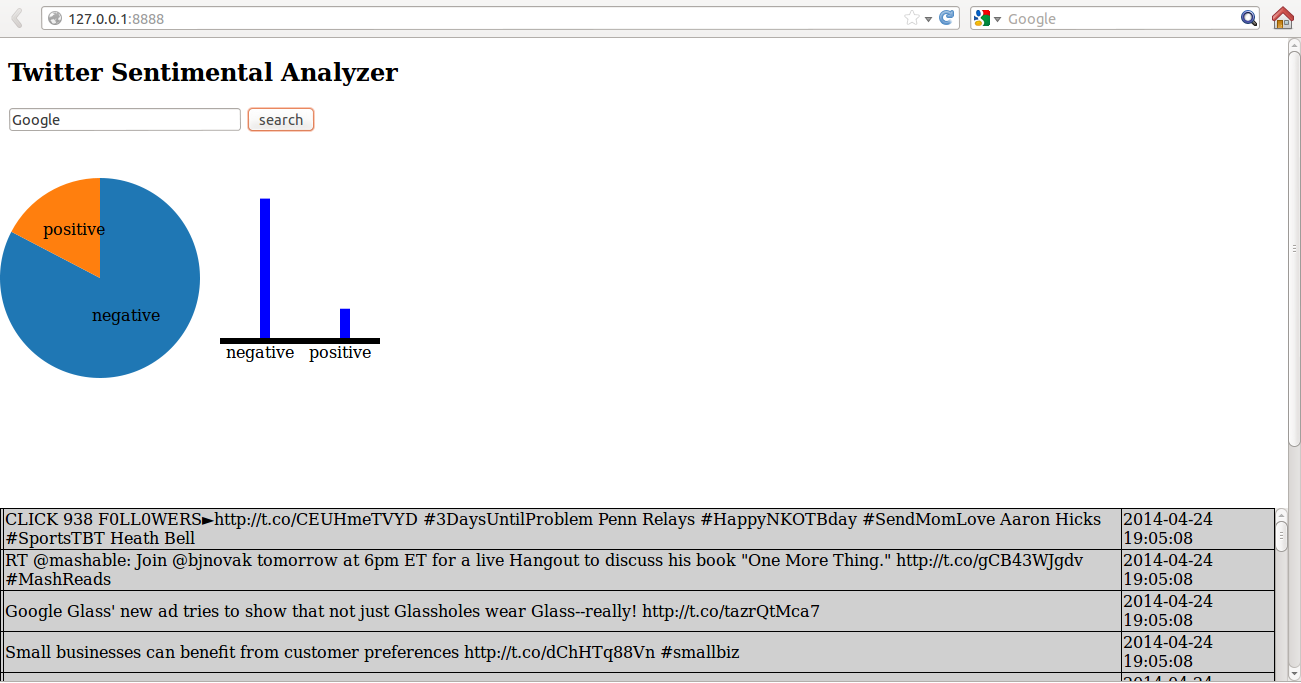
\includegraphics[width=1.0\textwidth]{pics/UI.png}
\caption{User Interface}
\label{Fig:ui}
\end{figure}

\subsection{Data Collection}
TwitterSearch\footnote{\texttt{\scriptsize{http://twittersearch.readthedocs.org/en/latest/‎‎}}} is a python-based interface which implements the Twitter Search API. 
\subsection{Online Analysis}
We analyzes each tweet using the naive bayes classifier and show the final statistics information in the pie chart and bar chart. The tweets will be shown in the table, where the negative tweet will shown in light gray while the positive tweet will be shown in light blue.

\begin{thebibliography}{9}
\bibitem{sentiment140}
  Alec Go, Richa Bhayani, Lei Huang.
  \emph{Twitter Sentiment Classification using Distant Supervision}.
  Stanford,
  Technical Report.

\bibitem{agarwal2011sentiment}
  Agarwal Apoorv, Xie Boyi, Vovsha Ilia, Rambow Owen, Passonneau Rebecca.
  \emph{Sentiment analysis of twitter data}.
  Association for Computational Linguistics,
  Proceedings of the Workshop on Languages in Social Media.

\bibitem{pang2002thumbs}
  Pang Bo, Lee Lillian, Vaithyanathan Shivakumar.
  \emph{Thumbs up?: sentiment classification using machine learning techniques}.
  Association for Computational Linguistics,
  Proceedings of the ACL-02 conference on Empirical methods in natural language processing-Volume 10.

\bibitem{codex}
  Qi Han, Junfei Guo, Hinrich Schuetze.
  \emph{CodeX: Combining an SVM Classifier and Character N-gram Language Models for Sentiment Analysis on Twitter Text}.
  Joint Conference on Lexical and Computational Semantics.

\bibitem{irbook}
  Christopher D. Manning, Prabhakar Raghavan and Hinrich Schütze.
  \emph{Introduction to Information Retrieval}.
  Cambridge University Press.

\end{thebibliography}
\end{document}
